\chapter{Descripteurs du mouvement}\label{chap:descripteurs}
Le mouvement humain est porteur d'informations, que ce soit lors d'une communication verbale \parencite{Huang2015SLR} ou non-verbale \parencite{Chang2013Pea}. Ces informations sont d'ordres différents et peuvent caractériser l'état psychologique de l'Homme (détection de l'émotion \parencite{Yuichi2007TEa} et de l'intention \parencite{Yu2015Hmb} ou décrire les interactions dans son environnement (reconnaissance d'actions \parencite{Kapsouras2014Aro}). Les gestes de la vie quotidienne (prendre un objet, s'asseoir, s'allonger, etc.) peuvent être détectés par des systèmes automatiques, tout comme leurs perturbations liées à un contexte émotionnel ou affectif (perturbation du geste lié à l'énervement, la compassion, etc.).

Si l'on se place dans un contexte d'analyse du geste, il faut être en mesure d'observer certaines caractéristiques du mouvement, relatives à, par exemple, la vitesse des articulations lors d'un lancer ou le déplacement du corps lors d'une danse, afin de pouvoir en extraire des informations pertinentes dans le contexte de l'analyse. Larboulette et Gibet définissent le geste comme une combinaison d'éléments multiples, associant le sens, le style et l'expressivité \parencite{larboulette2015Descriptors}. Le sens est décrit par un ensemble d'actions réalisées au sein du geste, permettant ainsi de définir l'objectif du mouvement. Le style est constitué des éléments propres à la personne effectuant le geste : sa morphologie, son genre, sa personnalité, ainsi que la manière d'effectuer le geste (se déplacer de manière gracieuse ou pesante, par exemple). L'expressivité englobe les nuances émotionnelles qui vont caractériser l'état d'esprit de la personne réalisant le geste.

Ces informations peuvent être déduites par analyse du mouvement brut capturé, en observant par exemple, les variations du même mouvement effectué dans le but d'accomplir la même tâche par différentes personnes. Si on considère une capture de « qualité » du corps humain (c'est-à-dire suffisamment de points de capture sur les parties du corps ciblées, à une fréquence suffisamment élevée, les valeurs acceptables de ces deux caractéristiques étant dépendantes de l'objectif d'apprentissage), il est alors possible de calculer, à partir des données brutes, des indicateurs exprimant des informations utiles pour l'apprentissage, en fonction des besoins d'analyse de la situation pédagogique. Ces indicateurs extraits sont nommés « descripteurs » dans la suite de ce manuscrit.

\section{Définition et principes}
Un descripteur est un indicateur calculé à partir du mouvement brut. Il est utilisé pour représenter des informations d'une partie ou de l'ensemble du corps, calculé à des temps \textit{t} précis ou selon un intervalle de temps pouvant aller jusqu’à la durée totale du mouvement. Un parallèle peut être fait avec la définition des indicateurs proposés par Choquet et Iksal : « des observables signifiant sur le plan pédagogique » calculés à partir de traces (tous types de données, générées à partir des interactions de l’étudiant avec le système) ou d'autres indicateurs \parencite{Choquet2007MTf}. Dans notre contexte, un descripteur permet de quantifier une ou plusieurs caractéristiques du mouvement, facilitant ainsi l'analyse manuelle ou automatique en diminuant, notamment, la quantité de données numériques à analyser. En effet, si l'on considère un e représentation d'un squelette constitué de 20 articulations lors d'un mouvement d'une durée de 15 secondes, enregistré à 60 postures par seconde, avec 3 valeurs pour la position (espace tridimensionnel) et 3 valeurs pour l'orientation (représentation d'Euler) de chaque articulation, on obtient ainsi le nombre suivant de données à analyser  $\overbrace{15}^{\text{temps}}*\overbrace{60}^{\text{nb frames}}*\overbrace{20}^{\text{nb articulations}}*\overbrace{3*3}^{\text{position et orientation}} = 162000$. De plus, les données de rotation sont souvent représentées sous forme de quaternion, de manière à pallier le problème du blocage de cadran (perte d'un degré de liberté resultant de la coplanarité de deux axes) propre à la représentation d'Euler \parencite{Kuipers2000QaR}, ce qui augmente le nombre de données obtenues. En conséquence, il est difficilement possible pour un humain de pouvoir observer, puis inférer des informations sur le mouvement à partir de l'affichage de ces valeurs numériques brutes. De plus, les informations sous forme d'un ensemble de positions et d'orientations nécessitent des connaissances scientifiques (au moins en géométrie) afin d'être interprétées. Le calcul de descripteurs à partir de données brutes a notamment pour objectif de réduire le nombre de valeurs à analyser, et de donner une nouvelle sémantique plus proche des connaissances de l'usager et de son vocabulaire métier, par utilisation des modèles sémantiques hiérarchiques ou de réification \parencite{Baudouin2008Rdt}. PAr exemple, à partir de la position, il est possible de calculer la distance d'écart entre deux membres, puis de qualifier l'amplitude du mouvement en fonction de valeurs seuils de la distance. De même, à partir de la position, il est possible de calculer des vitesses et des accélérations, puis de définir des valeurs seuil pour qualifier le mouvement comme un mouvement « régulier », « haché », « fluide » \textit{etc.} selon le vocabulaire métier.

Enfin, notons qu'il est possible d'extraire des descripteurs de mouvement à partir de deux types de données brutes principalement : (i) les squelettes (\textit{i.e.} ensemble de points capturés dans l'espace tridimensionnel, dont la chaîne articulaire a été reconstruite) capturés à l'aide d'une combinaison de capteurs inertiels, de caméra RGB-D ou de système de marqueurs avec des caméras infrarouges, et (ii), les images, c'est-à-dire des ensembles de pixels RGB ou nuage de points RGB-D provenant d'enregistrements vidéo. %Dans ce cas, il s'agit plus souvent d'inférence de descripteurs à partir de données moins précises. De plus, le squelette 3D peut aussi être reconstruit par estimation/approximation, augmentant le risque d'imprécisions du mouvement ainsi obtenu.

\section{Revues des descripteurs existants, classification et modèle de représentation}
Plusieurs travaux ont proposé de classer des ensembles de descripteurs du mouvement. Ces classifications ont souvent pour but de faciliter le choix d'un ensemble de descripteurs potentiels à partir des besoins d'analyse du geste : c'est le cas d'études telles que celles de Larboulette et Gibet \parencite{larboulette2015Descriptors} ou Morel \parencite{Morel2017Mts}. D'autres travaux s'intéressent au regroupement d'ensembles de descripteurs pertinents dans un contexte applicatif précis, par exemple la danse \parencite{Bouchard2007SSo}, l'écriture manuscrite \parencite{Delaye2013HBF}, \textit{etc.} Une présentation de différentes classifications de descripteurs, ainsi que de différents ensembles de descripteurs sont proposés dans cette partie.

\subsection{Descripteurs pour l'analyse de la performance}
Les travaux de Larboulette et Gibet \parencite{larboulette2015Descriptors} proposent de classer les descripteurs communément utilisés pour décrire le geste dans plusieurs autres études, selon plusieurs niveaux de regroupement : bas-niveau / haut-niveau, cinématique / géométrique, corps / environnement. La frontière bas-niveau / haut-niveau est définie par l'information donnée par le descripteur : un descripteur concernant des quantités cinématiques, dynamiques ou géométriques sera classé comme un descripteur bas-niveau, alors qu'un descripteur permettant d'exprimer des quantités exploitables dans une évaluation visuelle du mouvement ou par un expert sera considéré comme haut-niveau. La classification des descripteurs haut-niveau comme étant « exploitables » ne prend cependant pas en compte les connaissances de l'utilisateur final. La deuxième caractéristique propre aux descripteurs haut-niveau est qu'ils sont systématiquement calculés à partir de descripteurs bas-niveau, au même titre que les indicateurs de Choquet et Iksal sont calculés à partir des traces. Cette classification fournit également un formalisme mathématique homogène en posant une notation unifiée pour décrire le mouvement, les positions et les orientations à partir desquelles sont calculés les descripteurs. Ces travaux ne traitent cependant pas de l'utilisation possible de ces descripteurs, tant au niveau de l'analyse qu'il est possible d'en tirer (empirique ou non) que des cadres scientifiques ou applicatifs dans lesquels ils sont pertinents ou habituellement considérés. De plus, ces descripteurs nécessitent pour la majorité d'entre eux une connaissance scientifique poussée (biomécanique, par exemple) pour en tirer des informations utiles dans le cadre de l'apprentissage d'un geste.

Dans le cadre de son travail de thèse, Morel a également présenté une classification des descripteurs \parencite{Morel2017Mts}, en trois familles : les descripteurs reposant sur un modèle du corps humain, les descripteurs holistiques, qui utilisent la dynamique globale de l'objet considéré (corps humain ou autre), et les descripteurs locaux, caractérisant les mouvements à partir de points d'intérêt isolés. Pour chacune des familles, les descripteurs peuvent être calculés de manière à former une chaîne temporelle (« codage temporel », c'est-à-dire que le signal est codé à chaque instant) ou de manière globale (« codage global », un vecteur de caractéristiques représente le geste dans son entièreté). La famille des descripteurs reposant sur un modèle de corps humain est constituée des descripteurs de trajectoire, vitesse, accélération (linéaire ou angulaire), courbure, \textit{etc.} du mouvement. Sont également inclus les descripteurs géométriques, tels que les formes englobantes (cubes, ellipsoïdes, \textit{etc.}), et les descripteurs d'efforts, correspondant à l'effort déployé par une partie du corps sur l'intégralité du mouvement. La deuxième famille, celle des descripteurs holistiques, contient les descripteurs relatifs au mouvement de l'objet considéré dans sa globalité, sans s'intéresser aux spécificités dudit objet. Ainsi, vont être inclus les descripteurs calculés à partir de vidéos : zone en mouvement au sein de la vidéo, calcul d'une fonction d'énergie à partir des différences entre les images successives d'une vidéo, variation du gradient des images, \textit{etc.} Enfin, la troisième famille de descripteurs locaux se focalisent sur les points d'intérêts d'un objet, déterminés de manière automatique ou non. En observant le voisinage spatial ou temporel de ces points, il est ainsi possible d'obtenir des informations par rapport au mouvement de l'objet considéré. Des traitements visant à réduire les ensembles de descripteurs à un sous-ensemble sont également étudiés, tels que l'analyse en composantes principales (\textit{PCA}) ou la décomposition en valeurs singulières. Cette réduction conserve le même pouvoir discriminant pour la séparation des gestes par rapport à leurs caractéristiques initiales prédominantes. Bien qu'une étude analysant la pertinences de certains descripteurs en fonction de différents contextes applicatifs se trouve dans ce manuscrit, celle-ci ne concerne pas directement les familles de descripteurs proposées, ce qui fait qu'il n'est pas possible de directement mettre en contexte les descripteurs ou les familles et de proposer des cas applicatifs précis.

Il est intéressant de noter que le concept de bas-niveau / haut-niveau proposé par Larboulette et Gibet n'est ici pas un critère de séparation des descripteurs ; en effet, on retrouve des descripteurs bas-niveaux (\textit{i.e.} vitesse) et des descripteurs haut-niveau (\textit{i.e.} forme englobante) au sein d'une même catégorie. De plus, la classification de Morel mélange également des descripteurs issus de squelettes 3D et des descripteurs extraits de vidéos.

À l'origine de la description et la formalisation de mouvement humains, le système LBA (Laban Movement Analysis) est un système qui a beaucoup été utilisé, autant pour l'analyse que pour la séparation de gestes \parencite{Bouchard2007SSo}. L'objectif de ce système descriptif de gestes est de proposer une annotation hiérarchique dans l'objectif de caractériser originellement les mouvements de danse. Cette notation quantifie quatre informations sur le mouvement : sa direction, sa durée, la partie du corps concernée et sa dynamique. Les trois premières informations sont représentées par des signes (voir Fig. \ref{fig:laban_partition_et_directions_cinetographie}, en bas) et le placement de ces signes sur une portée défini la dynamique du mouvement (Fig. \ref{fig:laban_partition_et_directions_cinetographie}, en haut) : la succession des mouvements se lit sur l'axe vertical, de bas en haut, et les parties du corps concernées sont représentées sur l'axe horizontal. Ces travaux ont été les premiers à proposer un ensemble de descripteurs unifiés afin de décrire un geste dans sa continuité. Cependant, dans le contexte d'une opérationnalisation du système LBA, il est nécessaire de choisir et d'implémenter au préalable un ou plusieurs descripteurs de bas ou de haut niveau (au sens de la classification de Larboulette et Gibet) pour chaque dimension considérée du modèle, en fonction du mouvement à analyser.

\begin{figure}
    \centering
    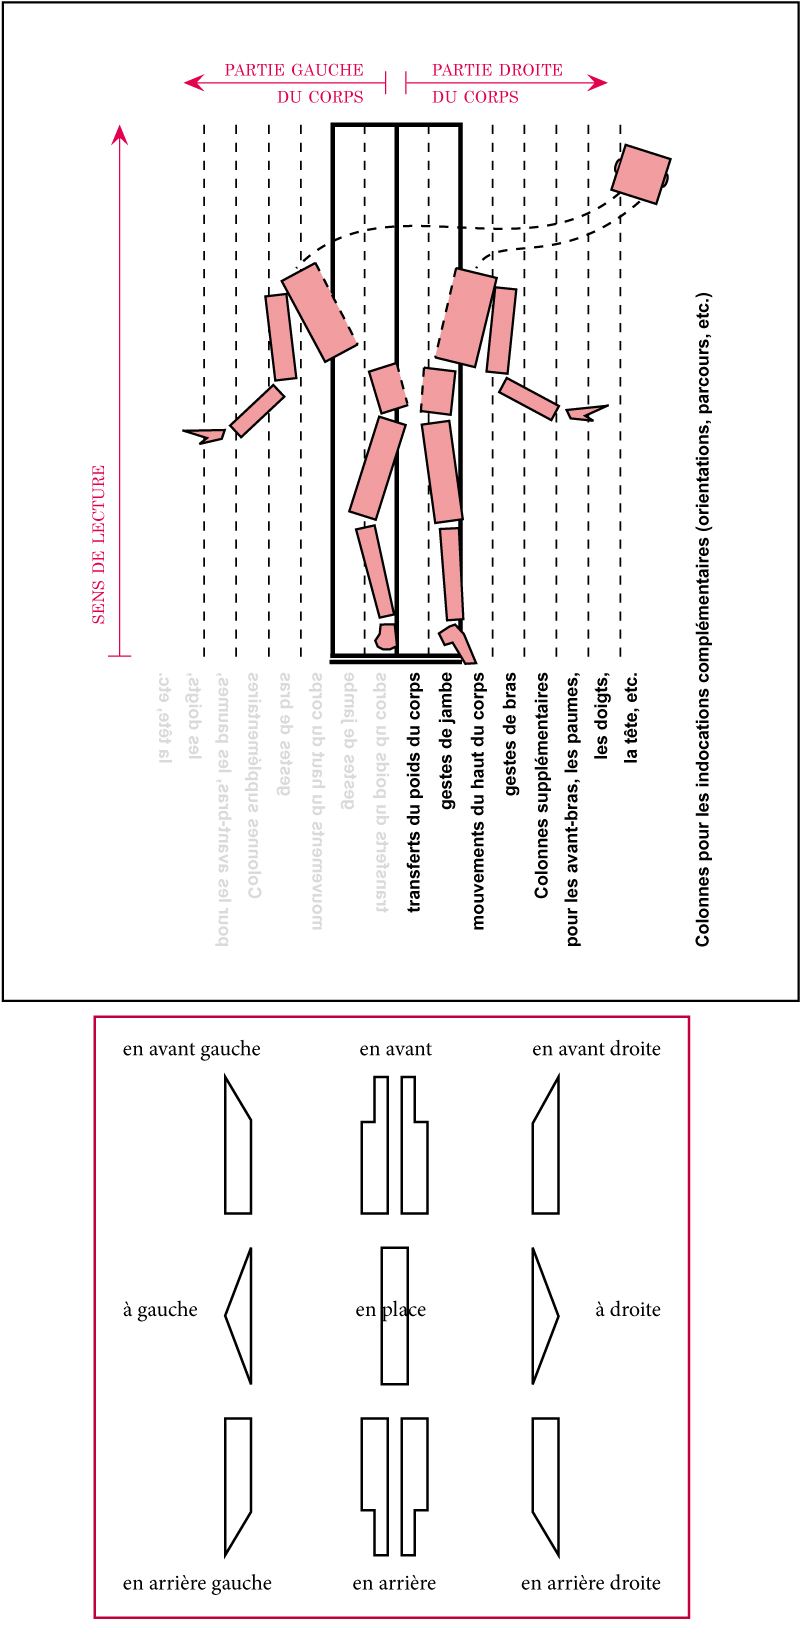
\includegraphics[width=\textwidth]{pictures/laban_partition_et_directions_cinetographie.png}
    \caption[Le système de partition de Laban]{Le système de partition de Laban. Ce système a été développé en premier lieu pour décrire les mouvements de danse. La lecture se fait de bas en haut, et chaque colonne correspond à une partie du corps. Dans chacune des colonnes, les indications de direction des parties du corps sont ajoutées. (Source: \parencite{WikiLaban})}
    \label{fig:laban_partition_et_directions_cinetographie}
\end{figure}

Aristidou \textit{et al.} proposent un ensemble de descripteurs caractérisant la danse folklorique selon quatre composantes du système de Laban, à savoir le corps, l'effort, la forme et l'espace \parencite{Aristidou2015FDE}. Les positions et les orientations, la hauteur du pelvis, la distance des jambes par rapport au sol et la taille des pas (distance entre les deux pieds) sont utilisés pour caractériser le corps. L'effort est divisé en quatre sous-catégories, possédants chacune deux polarités possibles : (i) l'espace occupé direct (précis et spécifique) ou indirect (non concentré sur un seul point), décrit à l'aide de l'orientation de la tête par rapport à la trajectoire du corps, (ii) le poids appliqué, fort ou léger, décrit à l'aide de la décélération du mouvement de la hanche, (iii) le temps, soudain (sentiment d'urgence, mouvement inattendu ou isolé) ou continu (réalisation du mouvement s'étalant dans le temps), décrit à l'aide de la vitesse et l'accélération du mouvement sur une période de temps prédéfinie, et (iv) le flux du mouvement, restreint (contrôlé, attentionné) ou libre (relâché, épanché, fluide), décrit à l'aide de la saccade du mouvement. La forme est décrite à l'aide du volume occupé par le corps de la personne, pris sur les cinq articulations extrêmes du corps (la tête, les mains et les pieds), la hauteur du torse, et la position des mains par rapport au corps. Enfin, l'espace est décrit à l'aide de la distance couverte par les hanches au court du temps, ainsi que l'aire correspondant à ce déplacement. L'organisation en quatre familles des descripteurs possède quelques similitudes avec la classification bas-niveau / haut-niveau qui est proposée dans les travaux de Larboulette et Gibet. Après extraction, les descripteurs de l'apprenant sont comparés avec ceux de l'expert, afin d'obtenir un score de corrélation correspondant à la similitude entre les deux gestes (Fig. \ref{fig:correlation_laban_descriptors}). Ce score, correspondant à la valeur absolue du coefficient de corrélation linéaire de Pearson, met en évidence les moments où le geste de l'apprenant est éloigné de celui de l'expert, mais ne propose pas une analyse sur les caractéristiques du mouvement à changer, malgré la précision des descripteurs utilisés. En conséquence, cette évaluation sous forme de score n'aide pas à l'amélioration de l'apprentissage du geste par l'apprenant.

\begin{figure}
    \centering
    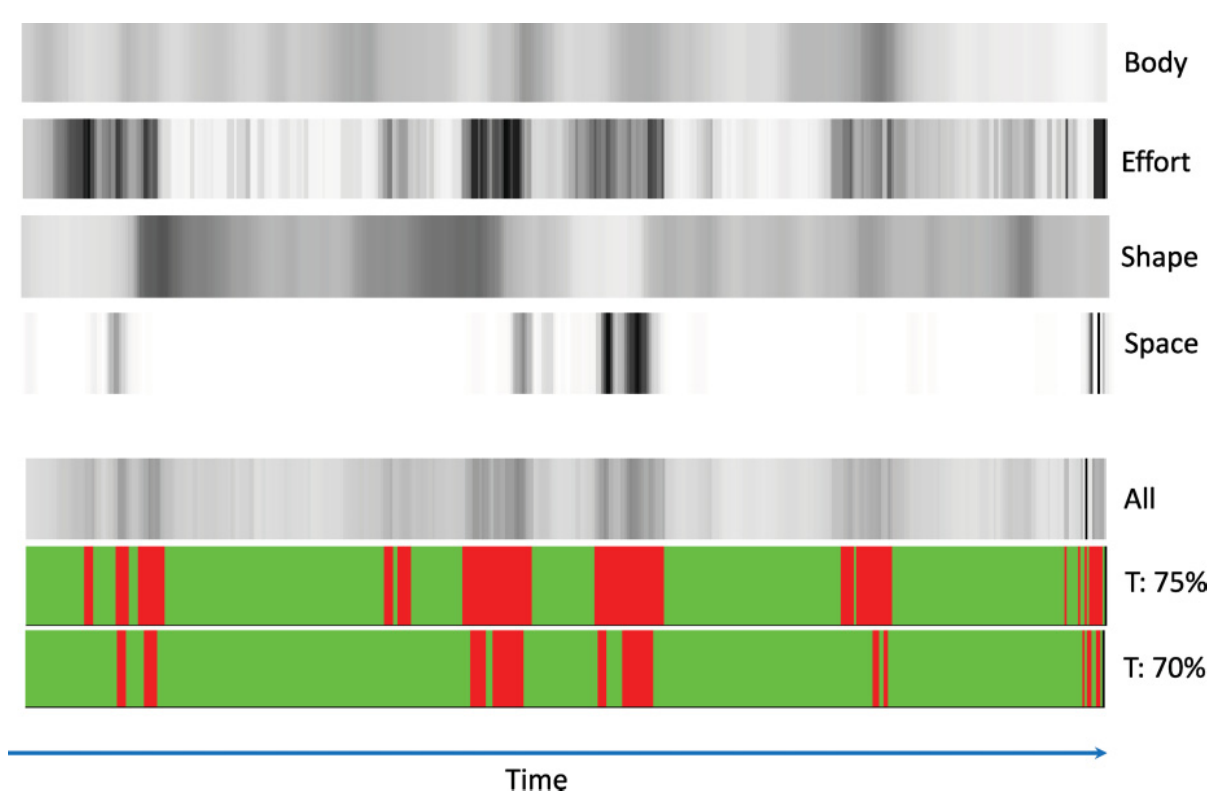
\includegraphics[width=\textwidth]{pictures/correlation_laban_descriptors.png}
    \caption[Corrélation entre le geste de l'apprenant et de l'expert]{La corrélation entre le geste de l'apprenant et de l'expert est calculée selon les quatre composantes du système de Laban considérées, puis moyennées. Le seuil $T$ choisi permet de changer la corrélation minimale à atteindre afin que le geste soit considéré comme bon. (Source: \parencite{Aristidou2015FDE}).}
    \label{fig:correlation_laban_descriptors}
\end{figure}

Toujours dans le domaine de la danse, Senecal \textit{et al.} utilisent un ensemble de descripteurs pour l'apprentissage de la salsa, selon trois axes : le rythme, l'interaction entre les partenaires et le style \parencite{Senecal2018MAa}. Ces descripteurs sont relatifs aux déplacements à effectuer lors de la danse. Ainsi, le rythme est évalué grâce à la position des pieds. Les valeurs successives de la norme de la vitesse des pieds attendues sont obtenues grâce à l'analyse du geste de l'expert. Le décalage entre les points d'inflexion de ce profil, correspondant à une nouvelle étape dans la suite de pas à réaliser, et ceux de l'apprenant permettent de mettre en évidence la synchronisation des pas avec la musique : un décalage temporel est ainsi obtenu. Le spectre du rythme de danse est ensuite extrait, à l'aide d'une transformée de Fourier, pour obtenir le décalage fréquentiel. L'interaction entre les partenaires est analysée sous trois angles : la corrélation du mouvement des jambes des deux partenaires, le décalage de rythme entre les deux partenaires, et enfin le décalage fréquentiel entre les deux partenaires. Enfin, le style est analysé à partir de l'aire couverte par la performance entière et la quantité de mouvement moyenne des hanches. Cette étude nécessite néanmoins d'extraire le tempo de la musique utilisée, dans le but d'obtenir un point de référence pour la synchronisation. Les descripteurs du mouvement sont donc complétés par une information temporelle supplémentaire non-relative au mouvement, celle des temps auxquels les percussions de la musique se font entendre. Ces données ne sont pas analysables sans connaissances en traitement du signal. Ainsi, il est impossible de présenter ces descripteurs sans une phase d'interprétation nécessaire pour tirer des conclusions sur le mouvement des apprenants. De plus, cette étude montre que malgré la sélection des descripteurs \textit{a priori} avec un expert, seuls quatre d'entre eux peuvent réelement aider à qualifier de manière satisfaisante le niveau des apprenants.

\subsection{Descripteurs pour l'indexation et la recherche de mouvements}
Les méthodes d'indexation et de recherche de mouvements cherchent à indexer les mouvements à l'aide de caractéristiques discriminantes, dans le but de de les stocker au sein d'une base de données. Le second objectif est de créer un langage de requête servant à retrouver et extraire efficacement et rapidement ces mouvement au sein d'une telle base de données.

Dans le cadre de la recherche de mouvements, Sakurai \textit{et al.} extraient un pentagone servant à représenter les postures du mouvement, à l'aide des données de position des articulations du squelette, dans l'optique de les comparer \textit{a posteriori} \parencite{Sakurai2015Ros}. Les données, capturées à l'aide d'une caméra Kinect™, sont prétraitées pour éliminer le bruit inhérent à ce type de capture. Ce traitement consiste à calculer, pour chaque posture, une moyenne sur les cinq postures adjacentes. Les postures sont ensuite normalisées, en harmonisant l'origine des repères, puis en divisant la longueur de chaque membre du corps par la taille du squelette. Un pentagone est ensuite extrait, reliant la tête, la main droite, le pied droit, le pied gauche et la main gauche. De ce polygone, trois aires différentes sont extraites, servant à représenter le mouvement (\ref{fig:polygons_areas}). La phase de recherche utilise ensuite l'algorithme de la Déformation Temporelle Dynamique (\textit{Dynamic Time Warping}, \textit{DTW}) pour calculer la distance entre le mouvement effectué et ceux présents au sein de la base de données. Cet algorithme permet de mesurer la similarité entre deux séries temporelles, ainsi que de les aligner, tout en s'affranchissant des contraintes temporelles. Plus formellement, l'algorithme du \textit{DTW} réalise un \textit{matching} entre les valeurs discrètes de deux séries temporelles. Si l'on prend l'exemple de deux personnes effectuant le même parcours, mais marchant à des vitesses différences,  la valeur du \textit{DTW} calculé entre ces deux séries temporelles sera élevée, indiquant une forte similitude entre ces deux séries, là où la distance euclidienne indiquera un écart élevé entre ces séries. Le mouvement stocké ayant la distance au sens du \textit{DTW} la plus petite est considéré comme étant le mouvement recherché. Afin d'évaluer les résultats, la métrique du \textit{F-score} est utilisée. Cette métrique est une combinaison de la Précision (P), qui correspond au ratio de de réponses correctes retournées par rapport au nombre total de réponses, et du Rappel (R), qui correspond au ratio de bonnes réponses retournées par rapport au nombre total de bonnes réponses. Les résultats des expérimentations montrent que, dans tous les cas, le descripteur basé sur les l'aire des quatre triangles extrait des mouvements enregistrés par la Kinect™ fourni le meilleur \textit{F-score}, par rapport aux deux autres descripteurs. Cette décomposition du mouvement en aires géométriques permet d'obtenir une performance de retour d'environ 71\% (au sens du \textit{F-Score}), environ 30\% plus faible que lors de l'utilisation de données capturées avec des systèmes de capture du mouvement plus précis. Les auteurs notent que cette différence peut être due à deux paramètres : la qualité des données obtenues (et donc, par extension, la méthode de filtrage appliquée) ainsi que le nombre d'aires extraites du polygone.

\begin{figure}
    \centering
    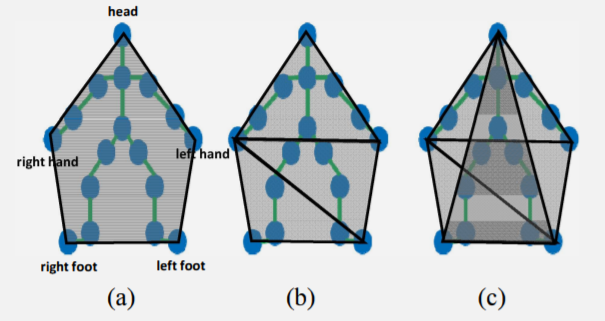
\includegraphics[width=\textwidth]{pictures/polygons_areas.png}
    \caption[Aires extraites du polygone du squelette \parencite{Sakurai2015Ros}]{Les trois descripteurs, constitués d'aires extraites du polygone englobant le squelette: (a) l'aire du polygone entier, (b) l'aire de trois polygones, (c) l'aire de quatre polygones (Source: \parencite{Sakurai2015Ros}).}
    \label{fig:polygons_areas}
\end{figure}

Xiao \textit{et al.} ont développé un système de descripteurs basés sur des postures 2D permettant de retrouver un mouvement à partir de dessins de postures-clés \parencite{Xiao2015Sbh}. Le mouvement est d'abord projeté sur 8 plans différents, de façon à passer d'une représentation 3D à plusieurs représentation 2D. Le système extrait ensuite des lignes reliant certaines articulations entre elles (les articulations extrêmes entre elles et les articulations extrêmes par rapport à la hiérarchie du squelette) servant à caractériser les articulations du corps à partir de leur distance relative, la direction de cette distance, la distance des articulations par rapport aux lignes et l'angle formé entre les différentes lignes (Fig. \ref{fig:skeletons_Xia}).

\begin{figure}[h]
    \centering
    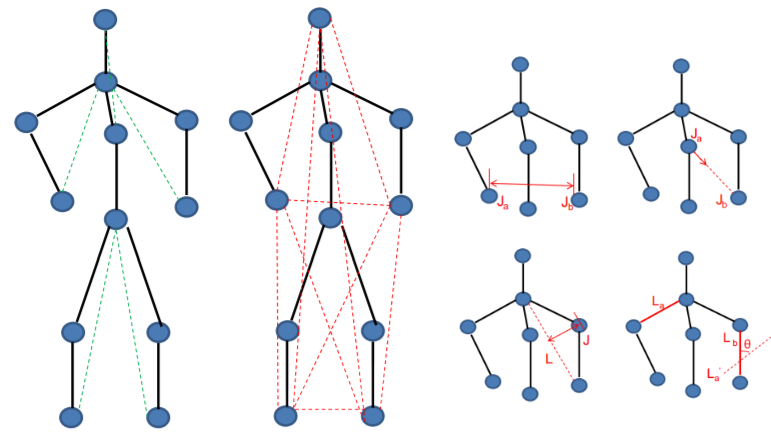
\includegraphics[width=\textwidth]{pictures/skeletons_Xia.png}
    \caption[Descripteurs basés sur les positions relatives des articulations entre elles \parencite{Xiao2015Sbh}]{Les descripteurs extraits caractérisent les postures par rapport aux distances relatives des articulations entre elles, ainsi qu'à leur distance et l'angle formé par rapport aux lignes reliant les autres articulations (Source: \parencite{Xiao2015Sbh}).}
    \label{fig:skeletons_Xia}
\end{figure}

Ces descripteurs sont ensuite réduits à un sous-ensemble, afin de limiter la redondance des informations contenues dans les données et d'améliorer les temps d'analyse \textit{a posteriori}. Pour cela, une méthode de sélection de caractéristiques semi-supervisée, basée sur le score Laplacien est utilisée. Ce score se base sur l'hypothèse que la projection des données dans un espace de caractéristiques réduits préserve la structure initiale de ces données \parencite{He2005LSf}. Le processus de recherche du mouvement se base sur un dessin fait à main levé par l'utilisateur. Le nombre de traits est limité à cinq, et le premier trait doit correspondre au torse. Grâce à ces contraintes, il est possible d'étiqueter automatiquement les articulations une fois le dessin terminé. La suite de postures dessinées par l'utilisateur est ensuite comparée à toutes les projections des mouvements présents dans la base de données à l'aide d'un algorithme des K plus proches voisins, et le mouvement le plus proche du dessin est récupéré (Fig. \ref{fig:posture_retrieval}).

\begin{figure}[h]
    \centering
    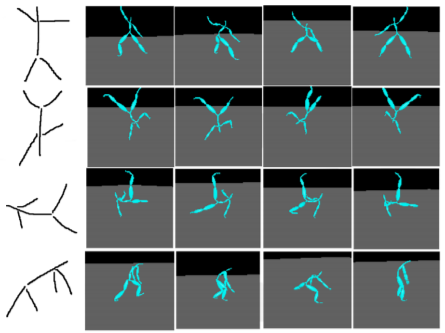
\includegraphics[width=\textwidth]{pictures/posture_retrieval.png}
    \caption[Mouvement retournés à partir de postures dessinées \parencite{Sakurai2015Ros}]{Quatre exemples de mouvement retournés à partir de postures dessinées à la main (Source: \parencite{Sakurai2015Ros}).}
    \label{fig:posture_retrieval}
\end{figure}

Les travaux cités ci-dessus proposent des ensembles de caractéristiques ayant pour but de stocker et de rechercher des mouvements de manière rapide et précise. Ces ensembles utilisent généralement une étape de sélection de caractéristiques, afin de réduire la dimensionnalité des données et ainsi d'accélérer le processus de recherche. Cette réduction peut cependant éliminer des descripteurs utiles à l'analyse du mouvement par un humain, et ainsi priver l'expert d'informations cruciales. En outre, la non prise en compte de l'utilisabilité, ni de la contextualisation de ces descripteurs par un humain fait que leur analyse peut être limitée en termes de retours possibles sur l'apprentissage d'un geste, voire impossible.


\subsection{Descripteurs pour la reconnaissance d'actions}
Certains travaux se focalisent sur l'extraction de descripteurs servant à identifier et séparer plusieurs actions. Dans ce cas, l'action peut soit concerner le corps entier (s'asseoir, prendre un objet, \textit{etc.}) ou des parties précises du corps (\textit{e.g.} reconnaissance d'écriture manuscrite).

 Ainsi, dans le cadre de la reconnaissance d'écriture, Delaye et Anquetil ont implémenté un ensemble de 49 descripteurs, nommé HBF49, liés à la manière d'écrire \parencite{Delaye2013HBF}. Ces descripteurs servent à caractériser les mouvements d'écriture, à l'aide : des points de début et de fin de trait, des angles formés par les différentes parties des lettres, de la proportion de trajectoires dirigées vers le bas, \textit{etc.} Cet ensemble de descripteurs a pour but de pallier les limites des ensembles de descripteurs existants pour l'écriture manuscrite. En effet, les travaux antérieurs ne permettent pas de caractériser toutes les informations pour ces gestes, car ils répondent souvent à un besoin d'observation et d'analyse précis, et aucune évaluation de référence n'a été conduite afin de les valider. Les tests effectués sur plusieurs jeux de données reconnus montrent que cet ensemble obtient un meilleur taux de reconnaissance de symboles que les jeux de descripteurs existants.

Dans le cadre de la reconnaissance d'actions, les travaux de Boulahia \textit{et al.} se basent en partie sur l'ensemble de descripteurs HBF49 et les généralisent à une trajectoire 3D dans l'environnement \parencite{Boulahia2016HIF}. Ces descripteurs ne posent aucune hypothèse sur les gestes considérés, et peuvent être utilisés pour n'importe-quel type de gestes. La validité de ce jeu de descripteurs pour décrire le mouvement, appelé HIF3D, a été testé sur deux jeux de données (HDM05 \parencite{HDM05Database} et UTKinect \parencite{UTKinectDatabase}) constitué de gestes non-techniques, et mis en concurrence avec d'autres ensembles de descripteurs déjà testés sur ces jeux de données (\textit{e.g.} SMIJ, Cov3DJ, HOJ3D). Il en ressort que les résultats sont meilleurs avec le jeu de descripteurs HIF3D.

Rao \textit{et al.} utilisent les moments d'inflexion dans la trajectoire, appelés instants dynamiques, afin de proposer une représentation des changements de trajectoire du geste, permettant ainsi de les segmenter en unités élémentaires \parencite{Rao2002VRR}. Les gestes utilisés dans l'étude sont des gestes du quotidien, \textit{e.g.} ouvrir et fermer un placard, prendre un objet, le poser, \textit{etc.} Ces unités élémentaires sont ensuite utilisées pour associer d'autres parties du mouvement, ou d'autres mouvements, à cette action. Ainsi, le système peut ensuite soit reconnaître une unité élémentaire comme étant similaire à une des unités élémentaires déjà visualisée, ou alors créer une nouvelle unité élémentaire si jamais celle-ci n'est pas suffisamment semblable à celles présentes dans le corpus. Cependant, la méthode ne se basant sur aucun apprentissage ou modèle pour segmenter et reconnaitre les mouvements, aucune sémantique n'est associée aux groupes d'unités élémentaires ainsi obtenus.


Des ensembles de descripteurs tel que HIF3D proposé par Boulahia \textit{et al.} couvrent beaucoup d'aspects différents du geste, offrant ainsi un bon taux de reconnaissance des actions. L'intégration de ces descripteurs à un système limite les besoins de réingénierie dans le cas de multiple domaines applicatifs, car il sont pensés pour être capable de reconnaitre une grande variété de mouvements. Cependant, beaucoup de ces travaux ne se focalisent pas sur l'apprentissage humain de mouvements. Ainsi, l'utilisation de ces descripteurs en tant qu'information descriptive humainement interprétable n'est pas prise en considération. Il n'est pas assuré que les descripteurs soient utilisables dans un processus d'analyse par un expert du geste ne disposant pas de connaissances scientifiques spécifiques à ces descripteurs.
%Le domaine de l'analyse de mouvement avec des données vidéo est également très riche en publications. Les descripteurs extraits à partir de vidéos peuvent être les mêmes que ceux extraits de données 3D; cependant, les méthodes de calcul ne sont pas les mêmes.

%En se basant sur les travaux de Laban, \parencite{Camurri2004AoE} proposent un système capable d'extraire une collection de descripteurs à partir d'enregistrements vidéo de mouvements. Le système permet de suivre le mouvement en temps réel et d'en extraire des descripteurs, mais également d'analyser la position occupée dans l'espace par la personne réalisant le geste, ainsi que l'extraction de trajectoires 2D à partir de la vidéo. Les descripteurs extraits des vidéos peuvent concerner des informations bas-niveau (trajectoire, vitesse, accélération) comme des informations haut-niveau (quantité de mouvement, orientation des parties du corps), selon la classification de Larboulette et Gibet \parencite{larboulette2015Descriptors}.

%Le domaine de l'étude de l'émotion chez l'humain utilise également de manière intensive des descripteurs, souvent extrait à partir du visage des personnes. Les émotions peuvent se lire à partir de plusieurs modalité du corps, mais les expressions faciales restent le moyen le plus efficace de les déterminer. Les travaux de \parencite{Ekman1978Fac} ont permis de créer le FACS (Facial Action Coding System), un ensemble de mouvements caractéristiques du visage, permettant de décomposer le mouvement en descripteurs. Ces descripteurs concernent les contractions (et décontractions), et sont appelés AU (action units). Ces descripteurs permettent de reconnaitre plusieurs émotions : la joie, la surprise, la tristesse, la colère, le mépris et le dégoût.

%Il est possible d'utiliser ces descripteurs dans un processus de classification, avec ou sans réduction de dimensionnalité \parencite{SanchezMendosa2015Erf}. Il est également possible d'obtenir des informations sur l'émotion à partir de descripteurs provenant du corps entier tels que la fluidité du geste, l'extension spatiale, la quantité de mouvement, \textit{etc.} reliés au niveau d'activation (dynamique de l'émotion) et d'évaluation (posititivé ou négativité) du geste \parencite{Malatesta2016Age}.


\subsection{Discussion}
Les travaux portant sur la classification des descripteurs ont pour but de créer des familles, afin de corréler chacune d'entre elles à un type d'analyse voulue. Ces classifications présentent des différences dans leur méthode de discrimination. Ainsi, Larboulette et Gibet \parencite{larboulette2015Descriptors} s'intéressent d'avantage à la séparation des descripteurs en termes d'origine des descripteurs : les descripteurs concernant la cinématique, la dynamique et la géométrie, calculés à partir du mouvement brut, sont dits de bas-niveau, et les descripteurs calculés à partir de descripteurs bas-niveaux sont dits de haut-niveau. Chez Morel \cite{Morel2017Mts}, la considération première est de séparer les descripteurs en fonction de l'objet en mouvement considéré. Ainsi, la première famille concerne les descripteurs représentant un corps humain en mouvement, la deuxième contient les descripteurs déterminant la dynamique d'un objet en mouvement, et la troisième contient les descripteurs concernant des points précis de l'objet considéré. Aristidou et Chrysanthou proposent une classification en fonction de la caractéristique du mouvement à considérer, entre le mouvement, l'effort, l'espace et la forme \parencite{Aristidou2014Fef}. Dans tous les cas, l'explicabilité des descripteurs calculés et l'utilisation de ces valeurs par des personnes expertes ou non n'est pas considérée. Ainsi, un expert du mouvement sans connaissances scientifiques poussées et un apprenant supposé novice dans le domaine ciblé ne pourront faire un usage direct de ces indicateurs.

Les travaux se focalisant sur un ensemble précis de descripteurs permettent de décrire les aspects du geste considérés dans l'étude \parencite{Senecal2018MAa} \parencite{Aristidou2015FDE} \parencite{Delaye2013HBF}. Ces ensembles offrent une analyse précise : par exemple, dans le cadre de l'écriture manuscrite, seront considérés non seulement la position de début et de fin de la main, mais également les différents traits effectués, les inflexions du poignet, le nombre de trait allant de haut en bas, \textit{etc.}. Les descripteurs présents dans ces études ont souvent une application limitée dans des contextes autres que le cadre applicatif choisi, bien que certains ensembles aient été pensés afin d'être réutilisable dans d'autres contextes \parencite{Boulahia2016HIF}. Quelque-soit la portée des descripteurs calculés,ils sont proposés soit à des systèmes d'analyse automatique \parencite{Aristidou2015FDE}, soit à des experts à-même d'en extraire des informations pertinentes dans le cadre de la réalisation ou l'apprentissage d'un geste \parencite{Senecal2018MAa}. Ainsi, la facilité d'utilisation de ces descripteurs par un non-expert n'est pas garantie, voire peu probable, comme dans les travaux de Senecal \textit{et al.} par exemple\parencite{Senecal2018MAa}.

L'utilisation des classifications et ensembles de descripteurs proposés dans des contextes annexes n'est pas assurée. En effet, bien que certains travaux proposent des ensembles pouvant couvrir une large gamme de caractéristiques du mouvement, dans le but de faire de la reconnaissance automatique, l'utilisation de ces descripteurs dans une situation d'apprentissage n'est pas considérée. Il en va de même pour les travaux portant sur l'indexation et la recherche de mouvements proposant des ensembles de descripteurs adaptés à ces deux fonctionnalités. De plus, les travaux portant sur l'indexation et la recherche de mouvements au seins de bases de données proposent des ensembles de descripteurs dont l'utilisabilité par un humain n'est pas considéré \parencite{Sakurai2015Ros} \parencite{Xiao2015Sbh}. En outre, ces ensembles peuvent présenter des redondances sémantiques, soit entre eux, soit au sein même du jeu de descripteurs considéré. Le calcul des descripteurs est une tâche qui peut prendre un temps non-négligeable, en fonction du nombre de données à traiter. La réduction des redondances au sein de ces jeux de descripteurs et la prise en compte des capacités de perception et d'interprétation des acteurs de l'apprentissage sont trois éléments importants à prendre en compte pour la conception d'un EIAH dédié à l'apprentissage de geste. La prochaine section propose une classification d'un ensemble de descripteurs réduit, issus de travaux présentés dans cette section, décrivant les différentes caractéristiques d'un mouvement. Cette nouvelle classification propose des cas d'usages et des domaines d'application, ainsi que les connaissances scientifiques nécessaires (ou non à leur utilisation).

\section{Classification de descripteurs élémentaires}\label{sec:class_descr}
Une nouvelle classification répondant à des besoins d'observation et d'analyse variés est proposée dans cette partie. Nous ne présentons ici que des descripteurs dit élémentaires, c'est-à-dire des descripteurs qui ne sont pas issus d'un calcul, d'une réinterprétation ou d'un ensemble de descripteurs « bas-niveau » du mouvement. Par exemple, Aristidou et Chrysanthou \parencite{Aristidou2014Fef} définissent la « hauteur de la hanche » comme descripteur. Cependant, ce descripteur provient de la composante verticale du descripteur « position 3D » de la hanche : Dans ce cas, le descripteur dit élémentaire est celui de la position selon l'axe vertical.

Chaque descripteur est caractérisé par son appartenance à une ou plusieurs des familles présentes dans le tableau \ref{descriptors_family}. Cette classification s'inspire des classifications déjà établies dans les travaux cités précédemment \parencite{larboulette2015Descriptors} \parencite{Morel2017Mts}. Les différentes familles proposées ne sont pas exclusives. De plus, la nécessité de posséder des connaissances scientifiques pour pouvoir contextualiser et interpréter le descripteur est indiquée, afin de donner des pistes quant à l'utilisation de ces descripteurs dans des contextes de retour à l'expert ou à l'apprenant.

Les colonnes « non-contigu, contigu et global » permettent de donner la possibilité d'obtenir la ou les valeurs du descripteur respectivement(i) sur des points précis (postures-clés), (ii) sur des postures qui se suivent temporellement ou (iii) sur la totalité du mouvement. Dans le premier et le deuxième cas, un vecteur de valeurs correspondant à un descripteur est retourné, dont la taille correspond soit au nombre de posture-clés, soit au nombre de postures successives choisies, et dans le dernier cas, un seul descripteur caractérisant l'ensemble du mouvement sera obtenu.

Les colonnes « cinématique » et « géométrique » donnent une indication sur la provenance du descripteur : un descripteur cinématique est directement dérivé à partir des propriétés du mouvement, alors qu'un descripteur géométrique proposera une information sur des aspects spatiaux du corps, voire son environnement.

La colonne « utilisation courante » met en évidence des domaines où ce descripteur est couramment utilisé, donnant ainsi des pistes quant à l'utilisation d'un descripteur en fonction du contexte applicatif fourni.

Enfin, la colonne « connaissance scientifique requise » indique si l'analyse de ce descripteur par un humain nécessite de posséder des connaissances scientifiques adéquates, ou si, à l'inverse, il est possible pour une personne sans connaissances particulières de comprendre et de tirer des informations utiles pour l'apprentissage du geste à partir de la valeur de ce descripteur.

Un même descripteur élémentaire présenté dans le tableau ci-dessus peut exprimer différentes caractéristiques d'un mouvement, en fonction de la fenêtre temporelle considérée. Ainsi, la vitesse prise sur un intervalle défini permet de suivre l'évolution de cette dernière lors d'un effort particulier, alors que la vitesse moyenne du mouvement prise globalement (moyenne des vitesses instantanées) donne une indication sur la rapidité du mouvement général. L'analyse de la position à un moment donné indique dans quelle position l'apprenant se trouve, alors que l'analyse de l'évolution de la position sur un temps donné résulte en l'obtention de la trajectoire de l'apprenant.

Le sens d'une partie des descripteurs proposés dans le tableau \ref{descriptors_classif} est explicité ici :

\begin{itemize}
	\item mouvement saccadé : donne une indication sur la fluidité du mouvement
	\item courbure : mesure la vitesse de changement de la trajectoire
	\item quantité de mouvement : moyenne pondérée des vitesses d'un ensemble d'articulation du corps
	\item forme englobante : plus petite forme (boîte, sphère, ellipsoïde...) englobant la totalité des articulations et des membres du corps
	\item enveloppe convexe : enveloppe minimale englobant le corps (Voir Fig. \ref{fig:convex_hull})
	\item centre de masse : moyenne pondérée (ou non) des positions des articulations (ou d'un sous ensemble des articulations) du corps
	\item équilibre : valeur booléenne indiquant si la projection du centre de masse au sol est comprise au sein de la projection au sol de la forme englobante du corps
	\item profilage : décrit l'évolution de la forme du corps au cours du mouvement : extension/rétractation, élargissement/réduction, enflement/creusement
	\item quantité d'effort : caractérise l'intensité d'un effort fourni sur un intervalle de temps défini, variant de « faible » à « intense »
	\item durée d'effort : représente la durée d'un effort fourni, caractérisé en « urgent » ou « continu »
\end{itemize}

\begin{figure}[h]
    \centering
    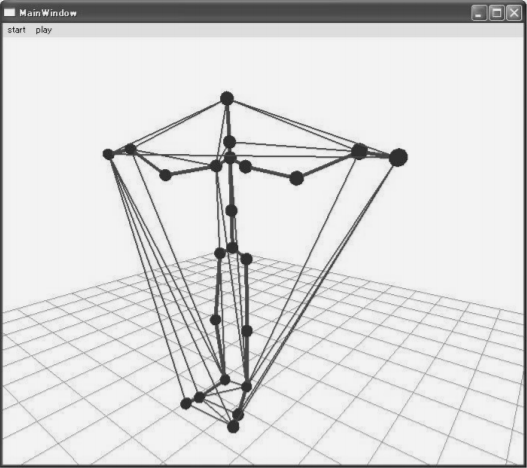
\includegraphics[width=6cm]{pictures/convex_hull.png}
    \caption[Enveloppe convexe]{L'enveloppe convexe correspond à la forme qui englobe le corps dans sa totalité, tout en gardant la distance minimale pour chaque segment la composant (Source: \parencite{Hachimura2005Aae})}
    \label{fig:convex_hull}
\end{figure}


\begin{landscape}
\centering
\begin{table}[]
\begin{tabular}{|l|l|l|}
\cline{1-3}
Type de descripteur & Description & Exemple \\ \cline{1-3}

Non contigu & \makecell[l]{calculé à des moments précis du mouvement\\(une ou plusieurs valeurs)} & Orientations prises à des postures clés\\ \cline{1-3}

Contigu & \makecell[l]{calculé sur une suite de postures contigües\\ (possiblement le mouvement entier)} & Vitesse au court du temps \\ \cline{1-3}

Global & \makecell[l]{une unique valeur qui définit une caractéristique du mouvement\\sur toute sa durée (une seule valeur)} & \makecell[l]{Périodicité du\\mouvement} \\ \cline{1-3}

\makecell[l]{Cinématique} & \makecell[l]{caractérise les aspects du mouvement relatifs au déplacement,\\la rotation, la vitesse, etc.                                                        } & Vitesse moyenne du mouvement\\ \cline{1-3}

Géométrique & \makecell[l]{caractérise des aspects relatifs aux parties du corps\\par rapport au corps tout entier ou à l'environnement} & \makecell[l]{Boîte englobante}\\ \cline{1-3}

\makecell[l]{Utilisation\\courante} & \makecell[l]{si un descripteur est souvent utilisé dans un domaine\\applicatif particulier} & \\ \cline{1-3}

\makecell[l]{Connaissance\\scientifique requise} & \makecell[l]{indique si le descripteur requiert des connaissances\\ scientifiques (physique, mécanique, géométrique, etc.) ou non\\pour être compris et utilisé dans un contexte particulier} & \\ \cline{1-3}
\end{tabular}
\caption[Différentes familles de descripteurs]{Différentes familles de descripteurs. Elles proviennent des travaux de Larboulette et Gibet \parencite{larboulette2015Descriptors} et Morel \parencite{Morel2017Mts}.}
\label{descriptors_family}
\end{table}
\end{landscape}

\begin{landscape}
\renewcommand{\arraystretch}{1.5}
\begin{table}[]
{\footnotesize
\begin{tabular}{c||c|c|c|c|c|c|c}
Descripteur & Contigu & Non-contigu & Global & Cinématique & Géométrique & \makecell[c]{Utilisation\\courante} & \makecell[c]{Connaissance\\scientifique\\requise} \\\hline
Position & X & X & & X & & Polyvalent & Géométrie \\\arrayrulecolor{gray}\hline
Orientation & X & X & & X & & Polyvalent & Géométrie \\\arrayrulecolor{gray}\hline
Durée & & & X & X & & Polyvalent & Non \\\arrayrulecolor{gray}\hline
\makecell[c]{Distance\\effectuée} & X & & X & & X & Polyvalent & Non \\\arrayrulecolor{gray}\hline
Vitesse & X & X & X & X & & Polyvalent & Cinématique du mouvement \\\arrayrulecolor{gray}\hline
Accélération & X & X & X & X & & Polyvalent & Cinématique du mouvement \\\arrayrulecolor{gray}\hline
\makecell[c]{Mouvement\\saccadé} & X & X & & X & & Analyse de la performance & Cinématique du mouvement\\\arrayrulecolor{gray}\hline
Courbure & X & X & & X & & Reconnaissance d'actions & Géométrie \\\arrayrulecolor{gray}\hline
\makecell[c]{Quantité\\de mouvement} & X & X & X & X & & Analyse de la performance & Dynamique du mouvement \\\arrayrulecolor{gray}\hline
Forme englobante & X & X & X & & X & Polyvalent & Géométrie \\\arrayrulecolor{gray}\hline
Enveloppe convexe & X & X & X & & X & Indexation et recherche & Géométrie \\\arrayrulecolor{gray}\hline
Centre de masse & X & X & X & & X & Analyse de la performance & Dynamique du mouvement \\\arrayrulecolor{gray}\hline
Équilibre & X & X & X & & X & Analyse de la performance & Non \\\arrayrulecolor{gray}\hline
Profilage & X & X & X & & X & Analyse de la performance & Dynamique du mouvement \\\arrayrulecolor{gray}\hline
Quantité d'effort & X & X & X & X & & Analyse de la performance & Dynamique du mouvement \\\arrayrulecolor{gray}\hline
Durée d'effort & X & & X & & & Analyse de la performance & Non
\end{tabular}
}
\caption[Classification des descripteurs élémentaires]{Une classification des descripteurs élémentaires de la littérature. Ils proviennent des travaux de Larboulette et Gibet \parencite{larboulette2015Descriptors} et Morel \parencite{Morel2017Mts}.}
\label{descriptors_classif}
\end{table}
\end{landscape}

En réduisant ainsi les descripteurs à un ensemble élémentaire, il est possible d'exprimer les descripteurs de plus haut-niveau par une combinaison de ces descripteurs. L'utilisation de cet ensemble pourrait ainsi, à terme, mener à la création d'un système de conception et d'intégration de descripteurs de haut niveau, calculables à partir des descripteurs élémentaires proposés et inteprétables par l'usager en fonction du contexte et de ses connaissances.



\section{Discussion}
Dans ce chapitre , nous avons étudié les descripteurs du mouvement calculables à partir des données capturées en fonction de leurs usages et des objectifs d’analyse. À partir de données de positions et d'orientations décrivant le mouvement de manière précise, il est possible d'extraire des informations caractérisant la forme, la position, la dynamique ou la cinématique du corps humain et du mouvement qui lui est associé. Il existe beaucoup de descripteurs pour caractériser le geste \parencite{larboulette2015Descriptors}. Cependant, ils sont majoritairement issus des descripteurs élémentaires présentés dans le tableau \ref{descriptors_classif}, soit d'une combinaison de plusieurs de ces descripteurs. Ainsi, il est en conséquence possible de réduire la large gamme de descripteurs utilisés dans l'analyse du mouvement à l'ensemble élémentaire présenté ici. L'utilisabilité de ces descripteurs par une personne non-experte, ainsi que les domaines applicatifs dans lesquels ils sont le plus souvent utilisés, sont considéré, afin de faciliter le choix des descripteurs en fonction des contextes applicatifs. L'implémentation de cet ensemble élémentaire au sein d'un système dédié à l'analyse de gestes permettrait de couvrir les besoins d'observations et d'analyse des utilisateurs, soit en calculant et en utilisant directement ces descripteurs, soit en combinant certains d'entre eux dans le but d'obtenir de nouveaux descripteurs.

Bien qu'il soit possible d'extraire ces descripteurs à partir de données de mouvement, ils ne sont néanmoins pas tous utiles en fonction du contexte. Ainsi, la pertinence des indicateurs est définie par les besoins d'observation et d'analyse des experts ou apprenants. La formalisation des besoins d'observation et d'analyse en descripteurs calculables est une étape cruciale afin de proposer des indications utiles sur le geste. Cette formalisation peut mener à la proposition d'un ensemble de descripteurs pertinent dans le cadre de l'analyse d'un mouvement. La problématique de formalisation de nouveaux descripteurs dans un système existant est rarement prise en compte dans les travaux existants. Cela peut s'expliquer par le côté \textit{ad-hoc} des systèmes extrayant des descripteurs du mouvement d'une part, et par la non-contextualisation des classifications de descripteurs d'autre part.

Il faut noter que le niveau de connaissance requis pour l'analyse des descripteurs est également lié au contexte. Ainsi, si l'on prend l'exemple d'une course à pied, le calcul et l'analyse conjointe de la durée et de la distance effectuée peuvent être suffisantes pour le pratiquant non spécialiste en biomécanique pour estimer sa performance physique. À l'inverse, l'analyse de la quantité d'effort ainsi que la durée de cet effort pour une partie précise du corps pourra être utilisée par un médecin afin d'évaluer les risques de blessures, mais sera difficile à interpréter pour une personne non-experte. L'analyse de ces données doit se faire dans un contexte précis, par un expert humain ou un système où la connaissance experte a été intégrée, pour être en mesure de donner du sens aux valeurs ainsi obtenues. Le prochain chapitre montre les différentes méthodes et techniques d'analyses possibles à partir de données de mouvement et des descripteurs.